\section{Научный текст} 
\begin{center}
\S5. Разбиение на смежные классы
\end{center}

Пусть $G$ - группа и $H$ - ее подгруппа. Будем говорить, что элементы $g_1,g_2 \in G$ \emph{сравнимы по модулю} $H$, и писать

\begin{center}
$g_1 \equiv g_2 (mod H)$            
\end{center}

\noindent если

\begin{equation}
g_1^{-1} g_2 \in H,
\end{equation}

\noindent т.е. $g_2 = g_1 h$, где $h \in H$. Это определение обобщает опредленеие сравнимости целых чисел по модулю $n$, которое получается в случае $G = \mathbb{Z}$, $H = n\mathbb{Z}$.
\par Докажем, что определенное таким образом отношение сравнимости по модулю $H$ является отношением эквивалентности:
\par 1) $g_1 \equiv g_2 (mod H)$, так как $g^-1 g = e \in H $;
\par 2) если $g_1 \equiv g_2 (mod H)$, т.е. $g_1^{-1} g_2 \in H$, то $g_2 \equiv g_1 (mod H)$, так как

\begin{center}
$g_2^{-1} g_1 = (g_1^{-1} g_2)^{-1} \in H$;
\end{center}

\par 3) если $g_1 \equiv g_2 (mod H)$ и $g_2 \equiv g_3 (mod H)$, т.е. $g_1^{-1} g_2, g_2^{-1} g_3 \in H$, то $g_1 \equiv g_3 (mod H)$, так как

\begin{center}
$g_1^{-1} g_3 = (g_1^{-1} g_2)(g_2^{-1} g_3) \in H$.            
\end{center}

Классы этой эквивалентности называются \emph{(левыми) смежными классами} группы $G$ по подгруппе $H$. Ясно, что смежный класс, содержащий элемент $g$, имеет вид
\eqref{formula1}:
\begin{equation} \label{formula1} gH = \{gh: h \in H\} \end{equation}

\noindent Одним из смежных классов является сама подгруппа $H$.
\par Поскольку умножение в группе не обязано быть коммутативным, мы получим, вообще говоря, другое отношение эквивалентности, взяв вместо условия \eqref{formula1} аналогичное ему условие

\begin{equation}
g_2 g_1^{-1} \in H.
\end{equation}

\noindent Классы этой эквивалентности называются \emph{правыми смежными классами} группы $G$ по подгруппе $H$. Они имеют вид \eqref{formula2}:
\begin{equation} \label{formula2} Hg = \{hg: h \in H\} \end{equation}

Заметим, что инверсия $g \mapsto g^{-1}$ устанавливает взаимно однозначное соответствие между множествами левых и правых смежных классов. А именно,

\begin{center}
$(gH)^{-1} = Hg^{-1}$.            
\end{center}

\begin{example}
Смежные классы аддитивной группы $\mathbb{C}$ по подгруппе $\mathbb{R}$ изображаются на комплексной плоскости прямыми, параллельными вещественной оси (рис. 1.1)
\end{example}

\begin{example}
Смежные классы мультипликативной группы $\mathbb{C^*}$ по подгруппе $\mathbb{R_+^{*}}$ положительных чисел - это лучи, исходящие из начала координат (рис. 1.2)
\end{example}

\begin{figure}[H]
\begin{multicols}{3}
\hfill
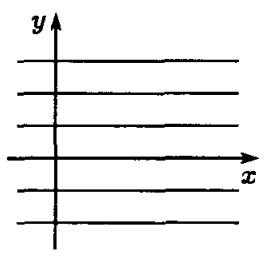
\includegraphics[width=45mm]{1.png}
\hfill
\caption{}
\label{figLeft}
\hfill
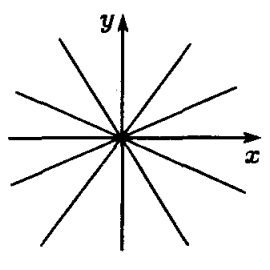
\includegraphics[width=45mm]{2.png}
\hfill
\caption{}
\label{figCenter}
\hfill
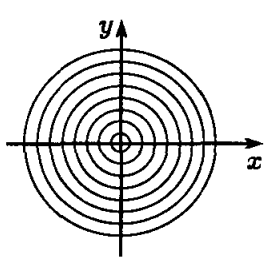
\includegraphics[width=45mm]{3.png}
\hfill
\caption{}
\label{figRight}
\end{multicols}
\end{figure}

\begin{example}
Смежные классы мультипликативной группы $\mathbb{C^*}$ по подгруппе
\begin{center}
$\mathbb{T} = \{z \in \mathbb{C^*}: |z| = 1\}$
\end{center}
- это окружности с центром в начале координат (рис. 1.3).
\end{example}

\begin{example}
В случае $G = GL_n(K), H = SL_n(K)$ условие (10), равно как и (11), означает, что $det g_1 = det g_2$. Поэтому левые смежные классы в данном случае совпадают с правыми (хотя группа $GL_n(K)$ не абелева); каждый из них представляет собой совокупность всех матриц с определителем, равным какому либо фиксированному числу.
\end{example}

\begin{example}
В группе $G = S_n$ рассмотрим подгруппу $H$, состоящую из подстановок, оставляющих на месте число $n$. Подстановки $\sigma_1, \sigma_2 \in S_n$ принадлежат одному левому смежному классу по $H$, если $\sigma_1^{-1} \sigma_2(n) = n$, т.е. если
\begin{center}
$\sigma_1(n) = \sigma_2(n)$.
\end{center}
\noindent Следовательно, имеется $n$ левых смежных классов $P_1,P_2, ..., P_n$, где
\begin{center}
$P_k = \{\sigma \in S_n: \sigma(n) = k\}$.
\end{center}
\noindent В то же время подстановки $\sigma_1, \sigma_2 \in S_n$ принадлежат одному правому смежному классу, если $\sigma_2\sigma_1^{-1}(n) = n$, т.е. если
\begin{center}
$\sigma_1^{-1}(n) = \sigma_2^{-1}(n)$.
\end{center}
\noindent Следовательно, имеется $n$ правых смежных классов $Q_1, Q_2, ..., Q_n$, где
\begin{center}
$Q_k = \{\sigma \in S_n: \sigma(k) = n\}$.
\end{center}
\noindent Мы видим, что правые смежные классы отличны от левых (за исключением $Q_n = P_n = H$).
\end{example}

Множество левых смежных классов группы $G$ по подгруппе $H$ обозначается через $G/H$. Число смежных классов группы $G$ по $H$ (левых или правх, безралично), если оно конечно, называется \emph{индексом} подгруппы $H$ и обозначается через $|G:H|$.

\newtheorem{Th}{Теорема}
\begin{Th}[теорема Лагранжа]
\emph{Если $G$ - конечная группа и $H$ - любая ее подгруппа, то}
\begin{center}
$|G| = |G:H||H|$
\end{center}
\end{Th}

\begin{proof}
Все смежные классы $gH$ содержат одно и то же число элементов, равное $|H|$. Поскольку они образуют разбиение группы $G$ (как классы эквивалентности), порядок группы $G$ равен произведению их числа на $|H|$.
\end{proof}

\newtheorem{Sl}{Следствие}
\begin{Sl}
\emph{Порядок любой подгруппы конечной группы делит порядок группы.}
\end{Sl}

Мы уже видели это в случае циклических групп.

\begin{Sl}
\emph{Порядок любого элемента конечной группы делит порядок группы.}
\end{Sl}

\begin{proof}
Это вытекакет из следствия 1 и того, что порядок элемента равен порядку порождаемой им циклической подгруппы.
\end{proof}

\begin{Sl}
\emph{Всякая конечная группа простого порядка является циклической.}
\end{Sl}

\begin{proof}
В силу следствия 1 такая группа должна совпадать с циклической подгруппой, порожденной любым элементом, отличным от единицы.
\end{proof}

\begin{Sl}
\emph{Если $|G| = n$, то $g^n = e$ для любого $g \in G$.}
\end{Sl}

\begin{proof}
Пусть ord $g = m$. В силу следствия 2 имеем $m | n$. Значит, $g^n = e$.
\end{proof}
\cite{учебник} 
\newpage
\section{Специальность}
\textbf Была создана таблица. Она состоит из следующих пунктов: номер пункта, специальность, ссылка на вакансию, заработная плата, требования(профессиональные), дисциплины из учебного плана, преимущества, недостатки. Ниже приведена таблица для специальности "Тестировщик". Краткий вывод по таблице: я не смог найти ни одну вакансию тестировщика без опыта, поэтому попасть на эту должность придётся постараться. Тем не менее, меня всё так же привлекает данная профессия.
\cite{ххру}

\newpage
\begin{landscape}
Таблица 3 - Тестировщик 
\begin{center}
\begin{tabular}{|p{1.3cm}|p{5cm}|p{2.6cm}|p{3cm}|p{3.2cm}|p{3.6cm}|p{2.8cm}|}
\hline
\textbf{\textnumero п/п} & \textbf{Ссылка на вакансию} & \textbf{Зарплата} & \textbf{Основные требования} & \textbf{Дисциплины, соответствующие требованиям} & \textbf{Преимущества} & \textbf{Недостатки} \\ \hline
1. &https://clck.ru/32Kqan&1150–1600\$ &Опыт работы в тестировании мобильных игр от года; Опыт составления и ведения тестовой документации; Грамотная письменная и устная речь; Желание развиваться в геймдеве
& Тестирование программного обеспечения; Программирование
 & Комфортные рабочие условия, гибкое начало рабочего дня; Прозрачные процессы, открытость данных аналитики; Профессиональная команда со стремлением разрабатывать качественные игры 
& Требуем ый опыт работы: 
1–3 
года.           \\ \hline
 2. & https://clck.ru/32KqiG & От 150 т. р. & Навык мануального тестирования интерфейса от 3 лет; Опыт тестирования API; Внимательность и системность; Минимальный опыт в автотестах и желание развиваться дальше  & Тестирование программного обеспечения; Программирование & Работа с крутой командой, где ваше мнение слышат и ценят, где дают обратную связь, поддержку, поле для реализации идей и ежедневную дозу юмора &Требуемый опыт работы: 3–6 лет
 \\ \hline
 
\end{tabular}
\end{center}
\end{landscape}

 \begin{landscape}
Продолжение таблицы 3
\begin{center}
\begin{tabular}{|p{1.3cm}|p{5cm}|p{2.6cm}|p{3cm}|p{3.2cm}|p{3.6cm}|p{2.8cm}|}
\hline
\textbf{\textnumero п/п} & \textbf{Ссылка на вакансию} & \textbf{Зарплата} & \textbf{Основные требования} & \textbf{Дисциплины, соответствующие требованиям} & \textbf{Преимущества} & \textbf{Недостатки} \\ \hline
 3.&https://clck.ru/32KqtG&50–100 т. р. & Понимание принципов тестирования и разработки; Опыт работы по Agile/Scrum методологии; Опыт работы с багтрекинговой системой; Умение разрабатывать тесткейсы & Тестирование программного обеспечения; Программирование &Работа в уникальном проекте, задачей которого является переосмысление рынка поставок телекоммуникацион ного оборудования в крупнейших странах мира& Требуем ый опыт работы: 1–3 года         \\ \hline
 4.&https://clck.ru/32KqiG&От 150 т. р. &Опыт тестирования API; Внимательность и системность&Тестирование программного обеспечения; Программирование  &ВРабота с крутой командой, где ваше мнение слышат и ценят&Требуемый опыт работы: 3–6 лет   \\ \hline
5. &https://clck.ru/32Kr8b&от 150 000 руб. &Знать основные методологии тестирования; Уметь анализировать результаты тестирования, ранжировать дефекты&Тестирование программного обеспечения; 
Программирование; Английский язык 
  &Работа в офисе в центре города или на удаленке с 10.00 до 19.00; адекватная заработная плата с возможностью роста 
& Требуемый опыт работы: 1–3 
года     
 \\ \hline
 
\end{tabular}
\end{center}
\end{landscape}



\newpage
\section{Заключение}
Первая глава содержит научный текст с формулами и рисунком. То есть навыки пользования Latex освоены. \par
Вторая глава работы демонстрирует анализ специальности мечты, содержит выводы по каждой вакансии, а также общий вывод про желаемую в будущем работу. Это помогло понять, каким темам стоит уделять внимание и к чему стремиться. \par
Таким образом, цель работы достигнута.